
\section{Design}
This section describes which object-oriented design approach we chose,
 what they are and which design patterns were used. The design for the
 Graphical User Interface (GUI) will also be covered.

		\subsection{Object-Oriented Design}
We chose to use both SOLID and GRASP as a guideline for object-oriented
 design. The reason behind using both, was due to public opinion that using
  one or the other was not
	sufficient.\footnote{http://forresterfootnotes.blogspot.dk/2013/03/solid-vs-grasp.html}\footnote{https://nikic.github.io/2011/12/27/Dont-be-STUPID-GRASP-SOLID.html}
  This way we could follow both guidelines where it was necessary, if
  SOLID did not help, GRASP just might and vice versa. Another reason
   was that the patterns of GRASP was used to assign responsibility to
    objects, whereas SOLID consist of programming principles that would
    help prevent bad code. SOLID and GRASP are described in the appendix \ref{appendix:SOLID} and \ref{appendix:GRASP}.
		\subsection{Design patterns}
In this subsection the most frequently used design patterns will be described.
 A design pattern is a reusable solution to a common problem.
			\subsubsection{Facades}
Facade design patterns help to simplify the communication between multiple
classes when used, by providing a collection of methods for common tasks,
 which also helps to make a complex system easier to understand. This pattern
 has been used to access the server, database, game mechanics and the GUI for all the windows.
The way this design pattern was used, it closely aligns to the Controller pattern in GRASP.
\\
\\
\textbs{Server}
\\
The server makes use of the DomainFacade in GeneralServices, whenever the
client needs to access it. It only includes the necessary methods such as
login, create account etc. Whereas a lot of the data is handled elsewhere,
 such as in the SecurityTokenService. This facade also includes the facade
 to the database, since the client does not need direct access to the database,
  but will instead go through this DomainFacade.
\\
\\
\textbs{Database}
\\
The database uses DatabaseFacade in GeneralServices, and includes simple
methods that holds the database code.
\\
\\
\textbs{Game Mechanics}
\\
The lobby uses DomainFacade in GameServices, and includes only the methods
the client would need to navigate the game once logged in, such as connect
and disconnect to the lobby, start matchmaking and take turn placing
 coordinates. The code that happens in between and after, is handled elsewhere.
\\
\\
\textbs{GUI}
\\
The GUI uses GUIFacade in the Client, which holds all the methods to
display events on the screen, such as placing a coordinate or changing the page.
			\subsubsection{Singleton}
The singleton design pattern ensures a class has only one instance.
This pattern has been used on most of the facades to ensure that all access
 in the system uses the same instances. An exception is the DatabaseFacade,
  since the access happens through the DomainFacade, so only a singleton
	 pattern on this facade is necessary.
\\
\\
For instance, the DomainFacade in GameServices, uses a singleton pattern
to ensure that the same lobby is used by all clients, and the GUIFacade uses
 it to ensure that only the clients’ own window is changed. The DomainFacade
  in GeneralServices uses it to ensure that the same SecurityTokenService access is used.
		\subsection{Graphical User Interface}
We chose to go with an easy to use graphical user interface, and only with the
 tools provided for the WPF windows such as buttons, listViews, labels etc. To
 make the GUI easy to use, the labels will clear when the user wants to input
  their data by clicking the label, and the buttons will be named appropriately
	 for the action it makes.
\begin{figure}[h]
	\centerline{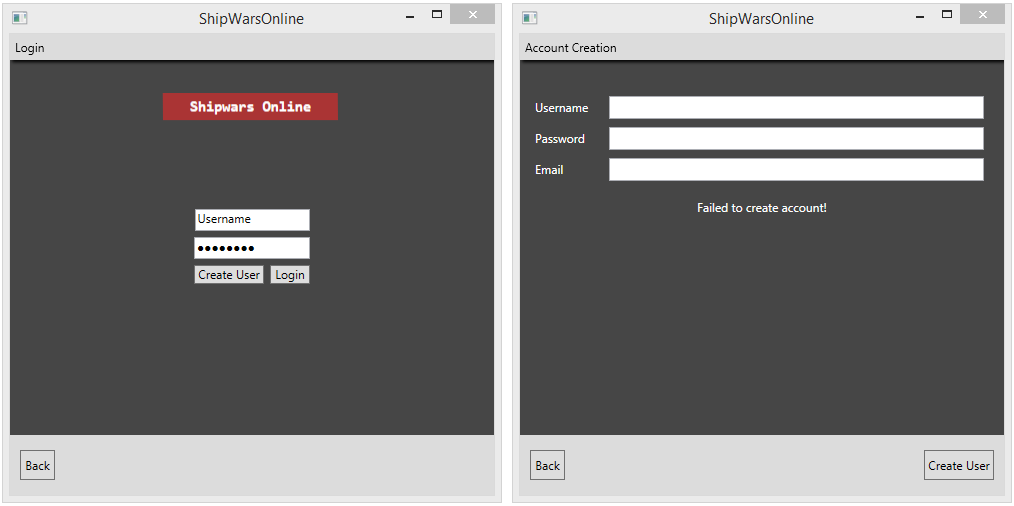
\includegraphics[scale=0.31]{GUILoginAccount}}
	\caption{Shows the Login and Account creation  page}
\end{figure}
\\
\textbs{Login page}
\\
The user will also be notified if the data is incorrect or missing, by
 displaying a label that describes the error when the button ‘Login’ has
  been pressed. If the data is correct, the user will be taken to the lobby
	page. The button ‘Back’ takes the user back to the previous page, and the
	 button ‘Create User’ takes the user to a page that allows them to create
	  an account.
\\
\\
\textbs{Account creation page}
\\
When the user clicks the ‘Create User’ button, an account will be created
and a label will be displayed saying that an account has successfully been
 created. If an error has occurred, the account will not have been created
 and a label describing the error will be displayed instead.
\begin{figure}[h]
	\centerline{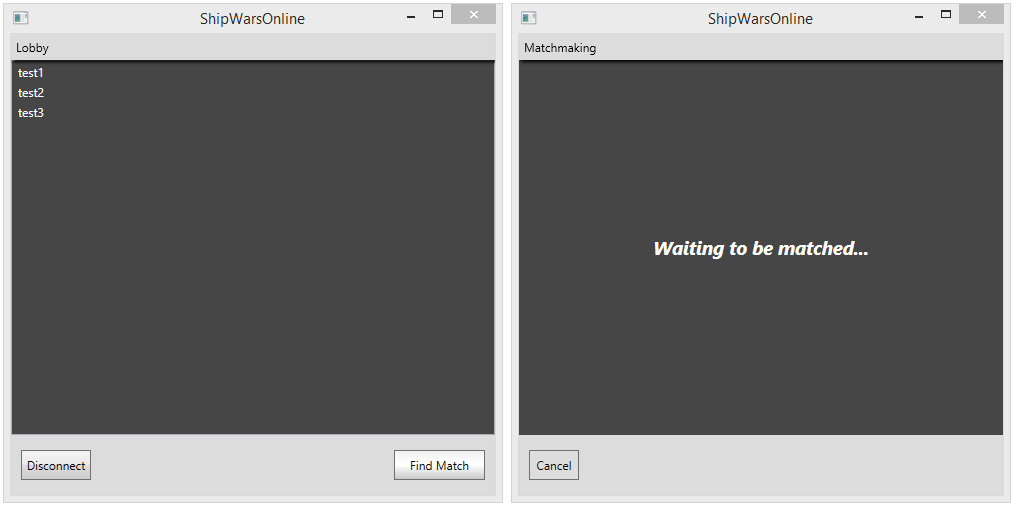
\includegraphics[scale=0.31]{GUILobbyWaiting}}
	\caption{Shows the Login and Account creation  page}
\end{figure}
\\
\textbs{Lobby page}
\\
From here the user becomes a player, and is displayed in a list with all
 the other players by their accounts usernames. This serves as a function to
 let the player know that other players are available, and whether or not a
  friend is online. The button ‘Disconnect’ serves the same purpose as the
	‘back’ button, with the additional functionality of actually disconnecting
	 the player from the game server. This means that the player will no longer
	  be displayed in the lobby and they become a user again by being taken back
		 to the Login page. The button ‘Find Match’ takes the player to the
		  matchmaking page.
\\
\\
\textbs{Matchmaking page}
\\
This page has not been made, and the player is instead transferred directly
 to waiting page. The original plan was to make a matchmaking page, where the
  player has the option to either search for a random available player, or a
	 specific player by their username. By clicking the ‘Random Player’ button,
	  the player would be taken to the waiting page. If the player clicked the
		‘Specific Player’, the system would check if the entered username is
		available, if true then both players would be taken to the game, if not
		 then a red label would be displayed specifying that the player doesn’t
		 exist or that the player is not online.
\\
\\
Since time has been a limit, this page was skipped, because the functionality
of a message system would have been needed. The message system would be there
 to notify the specific player for a match request, this player could then
 choose to respond with a yes or no, instead of being forced to play.
\\
\\
\textbs{Waiting page}
\\
This page is here to let the player know that the system is trying to find
an opponent, even though the page doesn’t have any functionality other than
 cancelling the action by clicking the ‘Cancel’ button, which then takes the
  player back to the find match page.
\\
\\
\textbs{Game page}
\\
When another player is available, the matchmaking system takes those two
 players and creates a game room, where the actual game is played. From here
  each player takes turns to place a tile on a coordinate, until someone wins.
	 The green field is the player's own, and the red is the opponent’s field.
	 The player would press the opponent's field to choose a coordinate, and then
	  press the ‘End Turn’ button. When a hit on a ship is made, it is displayed
		 in orange, a miss is blue, and when the ship is sunk it becomes red.
\begin{figure}[h]
	\centerline{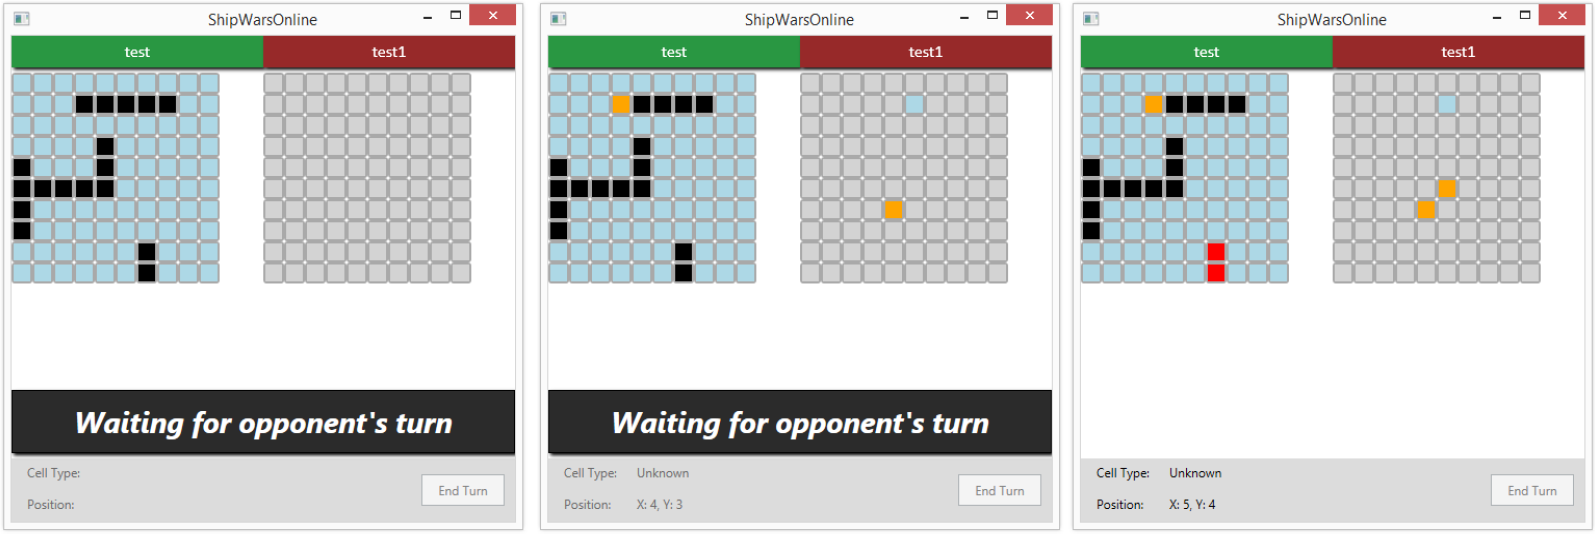
\includegraphics[scale=0.38]{GUIGame}}
	\caption{Shows the game GUI}
\end{figure}
\\
